\documentclass[11pt,a4paper]{article}
\usepackage[spanish,es-nodecimaldot]{babel}	% Utilizar español
\usepackage[utf8]{inputenc}					% Caracteres UTF-8
\usepackage{graphicx}						% Imagenes
\usepackage[hidelinks]{hyperref}			% Poner enlaces sin marcarlos en rojo
\usepackage{fancyhdr}						% Modificar encabezados y pies de pagina
\usepackage{float}							% Insertar figuras
\usepackage[textwidth=390pt]{geometry}		% Anchura de la pagina
\usepackage[nottoc]{tocbibind}				% Referencias (no incluir num pagina indice en Indice)
\usepackage{enumitem}						% Permitir enumerate con distintos simbolos
\usepackage[T1]{fontenc}					% Usar textsc en sections
\usepackage{amsmath}						% Símbolos matemáticos
\usepackage{listings}
\usepackage{color}

 
\definecolor{codegreen}{rgb}{0,0.6,0}
\definecolor{codegray}{rgb}{0.5,0.5,0.5}
\definecolor{codepurple}{rgb}{0.58,0,0.82}
\definecolor{backcolour}{rgb}{0.99,0.99,0.99}
 
\lstdefinestyle{mystyle}{
    backgroundcolor=\color{backcolour},   
    commentstyle=\color{codegreen},
    keywordstyle=\color{magenta},
    numberstyle=\tiny\color{codegray},
    stringstyle=\color{codepurple},
    basicstyle=\footnotesize,
    breakatwhitespace=false,         
    breaklines=true,                 
    captionpos=b,                    
    keepspaces=true,                 
    numbers=left,                    
    numbersep=5pt,                  
    showspaces=false,                
    showstringspaces=false,
    showtabs=false,                  
    tabsize=2
}
 
\lstset{style=mystyle, language=Java}

% Comando para poner el nombre de la asignatura
\newcommand{\asignatura}{Técnicas de los Sistemas Inteligentes}
\newcommand{\autor}{José María Sánchez Guerrero}
\newcommand{\titulo}{Práctica 1}
\newcommand{\subtitulo}{Desarrollo de un agente basado en búsqueda}

% Configuracion de encabezados y pies de pagina
\pagestyle{fancy}
\lhead{\autor{}}
\rhead{\asignatura{}}
\lfoot{Grado en Ingeniería Informática}
\cfoot{}
\rfoot{\thepage}
\renewcommand{\headrulewidth}{0.4pt}		% Linea cabeza de pagina
\renewcommand{\footrulewidth}{0.4pt}		% Linea pie de pagina

\begin{document}
\pagenumbering{gobble}

% Pagina de titulo
\begin{titlepage}

\begin{minipage}{\textwidth}

\centering

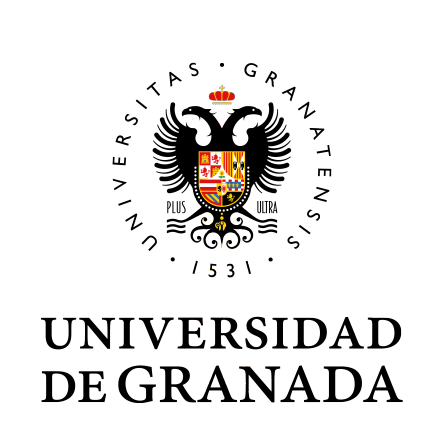
\includegraphics[scale=0.5]{img/ugr.png}\\

\textsc{\Large \asignatura{}\\[0.2cm]}
\textsc{GRADO EN INGENIERÍA INFORMÁTICA}\\[1cm]

\noindent\rule[-1ex]{\textwidth}{1pt}\\[1.5ex]
\textsc{{\Huge \titulo\\[0.5ex]}}
\textsc{{\Large \subtitulo\\}}
\noindent\rule[-1ex]{\textwidth}{2pt}\\[3.5ex]

\end{minipage}

\vspace{0.5cm}

\begin{minipage}{\textwidth}

\centering

\textbf{Autor}\\ {\autor{}}\\[2.5ex]
\textbf{Rama}\\ {Computación y Sistemas Inteligentes || Grupo 2 - Pablo Mesejo}\\[2.5ex]
\vspace{0.3cm}


\includegraphics[scale=0.3]{img/etsiit.jpeg}

\vspace{0.7cm}
\textsc{Escuela Técnica Superior de Ingenierías Informática y de Telecomunicación}\\
\vspace{1cm}
\textsc{Curso 2019-2020}
\end{minipage}
\end{titlepage}

\pagenumbering{arabic}
\tableofcontents
\thispagestyle{empty}				% No usar estilo en la pagina de indice

\newpage

\setlength{\parskip}{1em}


\section{Introducción}

La práctica consiste en implementar varios agentes que se puedan desenvolver adecuadamenete en los
distintos escenarios propuestos. Dispondremos de 5 mapas distintos, cada uno de ellos con un escenario
distinto.

\begin{itemize}
    \item En el primero simplemente tendremos que encontrar la salida
    \item En el segundo hay que recoger 10 gemas y luego salir
    \item En el tercero aguantar 2000 ticks del juego sin morir con un enemigo
    \item El cuarto aguantar 2000 ticks con varios enemigos
    \item El último será una fusión entre todos los otros, ya que hay que recoger 10 gemas y salir sin
          ser atrapado por ningun enemigo.
\end{itemize}

En mi caso he utilizado un algoritmo IDA* para encontrar los caminos más óptimos, y una técnica reactiva
que consiste en mantener al avatar lo más alejado posible de los enemigos en cada tick.


\section{Deliberativo}

Para nuestros agentes deliberativos vamos a utilizar, como hemos mencionado antes, el \textbf{algoritmo IDA*}.
He elegido este algoritmo porque está basado en el algoritmo base A* (es una extensión de este), sin embargo,
he decidido implementar IDA ya que obtiene los mismos resultados, pero no necesita almacenar todos y cada uno
de los posibles nodos candidatos. La gran ventaja que nos ofrece esto, es que reduce considerablemente el
consumo de memoria.

No obstante, pese a tener un consumo bajo en memoria, se podría haber implementado un algoritmo más eficiente
en cuanto a tiempo, sobre todo si tenemos en cuenta que disponemos 40 milisegundos por cada \textit{tick}. En
caso de que queramos calcular una ruta en este periodo de tiempo, puede ser que nos de error. En mi caso,
lo he dejado así porque los mapas son bastante pequeños y no muy complejos, por lo que no debería de tener
ningún problema; sin embargo, para mapas más difíciles sí que habría que mejorar su eficiencia.

A la hora de implementarlo, he necesitado dos clases. La primera es la clase ''\textbf{\textit{IDAStar.java}}'',
en la cual está implementado todo el algoritmo; y otra llamada ''\textbf{\textit{Node.java}}'', la cual
utilizamos para representar de una forma más sencilla cada una de las casillas del tablero adaptadas a nuestro
algoritmo. A continuación vamos a detallar cómo lo hemos hecho.

Empecemos con la clase \textbf{\textit{Node}} ya que la usaremos dentro de la otra. Lo primero es la declaración de
variables a utilizar:
\newline
\begin{lstlisting}
    // Valor heuristico del nodo actual
    private double hScore = Double.MIN_VALUE;
    // Coste del camino recorrido
    private double gScore = 0.0;
    // La suma de los valores anteriores
    private double fScore = 0.0;

    // Padre del nodo actual
    private Node parent;
    // Posicion en coordenadas (x,y) del nodo actual
    private Vector2d position;
\end{lstlisting}

Como es un algoritmo basado en el A*, tenemos que poner las 3 variables características de éste: $f()=g() + h()$.
Junto a ellas, también hay que poner la posición en coordenadas $(x,y)$ del nodo actual, y otra variable para
el padre, es decir, la posición de la cual se ha generado.

He añadido un constructor para poder crear un nuevo nodo a partir de una variable \textit{Vector2d}, que
representa una posición concreta en el mapa. Para acceder y modificar todas estas variables tendremos sus
correspondientes métodos \textit{getX()} y \textit{setX(value)}.

Implementaremos las siguientes funciones que nos podrán ser útiles en determinadas situaciones. Para comparar
un nodo con otro, es decir, comparar los valores de \textit{f()}, he añadido una función que devuelve -1, 1 o 0
dependiendo de si es menor, mayor o igual al nodo a comparar, respectivamente. Tenemos otra función que nos
dirá si un nodo es igual a otro (no en cuanto al valor de \textit{f()}, sino al estado de los nodos). Para
obtener los nodos sucesores del nodo actual, la cual inserta en una lista los nodos correspondientes a las
casillas que rodean a la actual, comprobando antes que esta casilla sea transitable, es decir, no sea un
obstaculo. Por último, tenemos la función que determina la \textit{h()}. Como estamos en un mapa cuadriculado,
la distancia al padre siempre va a ser 1.

Una vez hemos terminado con la clase \textit{Node}, vamos a pasar a la clase \textbf{\textit{IDAStar}}. En
ella tenemos las siguientes variables:
\begin{lstlisting}
    // Creamos las variables para los nodos

    // Nodo inicial desde donde saldra nuestro avatar
    private Node initialState;
    // Nodo objetivo para el camino
    private Node goalState;
    // Posiciones de los obstaculos del mapa
    private ArrayList<Vector2d> tiposObs;

\end{lstlisting}

Aqui también tenemos un constructor para que nos genere un camino a partir del nodo inicial, otro final y una
lista con las posiciones de los objetos por las que no puede pasar nuestro avatar.

La primera función más relevante de esta clase es \textbf{\textit{search()}}, en la cual comienza la
búsqueda. En ella realizaremos una búsqueda recursiva (que detallaremos posteriormente), hasta que la cota
hallada sea 0, o lo que es lo mismo, hasta que hayamos llegado al objetivo. Devuelve un $Node$ que es el
último nodo de la ruta óptima. Devolverá nulo si no se puede encontrar el nodo objetivo.

Ahora vamos a pasar a la función \textbf{\textit{recursive\_search()}}, la cual es la que maneja todo
el algoritmo y encuentra el camino óptimo desde dentro de la función \textit{search()}. Ésta busca recursivamente
los hijos de los nodos, evitando buscar el camino hacia abajo con una $f$ más alta que el límite $f$ actual.
Si se encuentran caminos con un limite más alto, devolverá la $f$ más pequeña sobre el límite encontrado.
Este límite sobre el $f$ mas pequeño es un nuevo límite $f$ potencial durante la próxima iteración. La función
devolverá 0 si se encuentra el nodo objetivo e Integer.MAX\_VALUE si no se puede encontrar el nodo objetivo.

Por último, tenemos una función \textit{\textbf{getPath()}} que devuelve una lista de nodos que representa el
camino óptimo. Como hemos mencionado, la función \textit{search()} sólo devuleve el nodo final, asi que esta
función se encargará de pasar por todos los padres del último nodo e insertalos en la lista, hasta llegar al
nulo.

Con esto ya hemos terminado de explicar las clases y funciones auxiliares que utilizaremos para los modelos
deliberativos, asi que pasemos a ver el funcionamiento de ambos.


\subsection{Deliberativo simple}

Antes de ejecutar el \textit{act} (en este y en todos los agentes), se inicializan las variables correspondientes
al factor de escala, posición del avatar, portal, objetos, muros, etc\dots; y en el caso del deliberativo, también
inicializamos y calculamos el path. Esto lo hacemos aquí, porque tenemos más margen de tiempo que en el \textit{act},
donde sólo tenemos 40 milisegundos para tomar una decisión.

La ventaja que tenemos en este agente deliberativo simple, es que no es necesario recalcular ningún path, por
lo que el obtenido en un principio es que nos servirá hasta el final. Finalmente, lo único que tendremos que
hacer en el \textit{act} es obtener el primer elemento del camino calculado (siguiente posición del avatar),
calcular el siguiente movimiento a partir de él y devolver su acción correspondiente.


\subsection{Deliberativo compuesto}





\newpage

\section{Reactivo}

\subsection{Reactivo simple}

\subsection{Reactivo compuesto}



\newpage

\section{Deliberativo-Reactivo}


\end{document}